\documentclass[areasetadvanced]{scrartcl}

\usepackage[utf8]{inputenc}
\usepackage[T2A]{fontenc}
\usepackage[english,russian]{babel}
\usepackage{booktabs}
\usepackage[footskip=1cm,left=25mm, right=15mm, top=20mm, bottom=20mm]{geometry}
\usepackage{setspace}
\usepackage{amsmath, amssymb}
\usepackage{graphicx}
\usepackage{tikz}
\usetikzlibrary{arrows.meta}
\usepackage{float}
\usepackage{dashrule}
\usepackage{fancyhdr}
\usepackage{hyperref}
\usepackage{parskip}
\usepackage{textcomp, enumitem}
\usepackage{indentfirst}
\usepackage{algorithm}
\usepackage{algpseudocode}
\usepackage{array}
\usepackage{afterpage}
\usepackage{minted}
\setcounter{secnumdepth}{3}
\setcounter{tocdepth}{3}
\usepackage{listings}
\setlength{\parindent}{1.25cm}

\tikzstyle{block} = [rectangle, rounded corners, minimum width=3cm, minimum height=1cm, text centered, draw=black, fill=lightgray]

\setkomafont{sectioning}{\normalfont\bfseries}
\setkomafont{section}{\normalfont\Large\bfseries}
\setkomafont{subsection}{\normalfont\large\bfseries}
\setkomafont{subsubsection}{\normalfont\large\bfseries}
\setkomafont{paragraph}{\normalfont\large\bfseries}

\lstset{
  language=Python,
  basicstyle=\ttfamily\small,
  keywordstyle=\color{blue}\bfseries,
  stringstyle=\color{red},
  commentstyle=\color{green!70!black},
  numbers=left,
  numberstyle=\tiny,
  stepnumber=1,
  numbersep=10pt,
  showstringspaces=false,
  breaklines=true,
  frame=single
}

\setcounter{tocdepth}{2}
\begin{document}
\sloppy
	\thispagestyle{empty}
	\begin{center}
		\large{МИНОБРНАУКИ РОССИИ} \par
		\vspace{0.3cm}
		\normalsize
		{ФЕДЕРАЛЬНОЕ ГОСУДАРСТВЕННОЕ АВТОНОМНОЕ ОБРАЗОВАТЕЛЬНОЕ УЧРЕЖДЕНИЕ ВЫСШЕГО ОБРАЗОВАНИЯ} \par
		\vspace{0.3cm}
		\textbf{\guillemotleft САНКТ-ПЕТЕРБУРГСКИЙ ПОЛИТЕХНИЧЕСКИЙ}
		\textbf{УНИВЕРСИТЕТ ПЕТРА ВЕЛИКОГО\guillemotright} \par
		\vspace{0.3cm}
		{Институт компьютерных наук и кибербезопасности}\par
		{Высшая школа технологий искусственного интеллекта}\par
	\end{center}
	\vfill
	\begin{center}
		{\large Отчёт по дисциплине \guillemotleft Алгоритмические основы компьютерной графики\guillemotright}\par
		{\huge Лабораторная работа №2 
		
		\guillemotleft Алгоритм отсечения отрезка выпуклым телом. Алгоритм Кируса-Бека\guillemotright}\par
            {\huge Вариант \textbf{№14}}
         
	\end{center}
	\vfill
	\begin{flushleft}
		Студент: \hspace{1.8cm} \rule[0pt]{2.5cm}{0.5pt}\hfill Салимли Айзек Мухтар Оглы\par
		\vspace{1.5cm}
		Преподаватель: \hspace{0.55cm} \rule[0pt]{2.5cm}{0.5pt}\hfill Курочкин Михаил Александрович
	\end{flushleft}
	\vspace{0.5cm}
	\begin{flushright}
		\guillemotleft \rule[0pt]{0.8cm}{0.5pt}\guillemotright \rule[0pt]{2cm}{0.5pt} 20\rule[0pt]{0.5cm}{0.5pt} г.
	\end{flushright}
	\vfill
	\begin{center}
		Санкт-Петербург, 2025
	\end{center}
	\newpage
	\tableofcontents
	\newpage
\section*{Введение}
	\addcontentsline{toc}{section}{Введение}
    Алгоритм Кируса–Бека (Cyrus–Beck) — это один из классических алгоритмов отсечения отрезков, применяемых в компьютерной графике. Он основан на параметрическом представлении отрезка и векторной геометрии, что делает его особенно подходящим для работы с выпуклыми многоугольниками и многогранниками.

Данный алгоритм применяется в следующих областях:

\begin{itemize}
    \item \textbf{Компьютерная графика:}
    \begin{itemize}
        \item Отсечение лишних отрезков и линий за пределами видимой сцены (clipping);
        \item Подготовка сцен к рендерингу, особенно в 2D и 3D-графике.
    \end{itemize}
    
    \item \textbf{Геометрические алгоритмы:}
    \begin{itemize}
        \item Проверка принадлежности точки/отрезка выпуклому многоугольнику;
        \item Расчёт пересечений отрезков с границами объектов.
    \end{itemize}
    
    \item \textbf{Системы автоматизированного проектирования (CAD):}
    \begin{itemize}
        \item Удаление невидимых линий;
        \item Обработка контуров и сложных геометрий.
    \end{itemize}
\end{itemize}

На данный момент алгоритм Кируса–Бека используется в следующих случаях:

\begin{itemize}
    \item При необходимости высокой точности и контроля над отсечением, особенно в научных и инженерных приложениях;
    \item Когда нужно работать с выпуклыми полигонами и важно строго учитывать направление нормалей;
    \item При разработке собственных графических движков или low-level алгоритмов, где важно понимать и контролировать всю геометрию вручную.
\end{itemize}
В данном отчете проведена реализация и сравнение алгоритма отсечения отрезка выпуклым телом (Кируса-Бека) с библиотечным алгоритмом Shapely.\\ 

Также в отчете теоретически сравнивается алгоритм Кируса-Бека с другими алгоритмами отсечения отрезка выпуклым телом, рассмотрены такие алгоритмы как:
\begin{itemize}
    \item Алгоритм Коэна-Сазерленда
    \item Метод пересечения с полуплоскостями
\end{itemize}
\newpage
\section{Постановка задачи алгоритма Кируса-Бека}
\begin{itemize}
    \item Дано: \(\mathbf{p0}\), \(\mathbf{p1}\) — отрезок, \(\text{polygon} = (\mathbf{v}_1, \mathbf{v}_2, \dots, \mathbf{v}_n)\) — выпуклый многоугольник.
    \item Надо: Найти \(\mathbf{q0}\), \(\mathbf{q1}\) — точки пересечения отрезка и многоугольника.
    \item Ограничения: \(\text{polygon}\) — выпуклый, отрезок \(\mathbf{p0}\mathbf{p1}\) пересекает \(\text{polygon}\).
\end{itemize}
\newpage
\section{Математическое описание алгоритма Кируса-Бека}
Пусть требуется отсечь \textbf{отрезок} с начальными и конечными точками 
\(\mathbf{p0}\) и \(\mathbf{p1}\) относительно выпуклого многоугольника \(\text{polygon}\).
Введём \textbf{параметрическое} уравнение для любой точки \(\mathbf{p}(t)\)
на прямой, содержащей этот отрезок:
\[
\mathbf{p}(t) = \mathbf{p0} + t(\mathbf{p1} - \mathbf{p0}), 
\quad t \in [0,1].
\]

Здесь \(t = 0\) соответствует точке \(\mathbf{p0}\), а \(t = 1\) — точке 
\(\mathbf{p1}\). Если после выполнения алгоритма окажется, что допустимый диапазон 
\(t\) сузился до \([\ t_{\min},\, t_{\max}\,]\subseteq[0,1]\), то отсечённая часть 
отрезка будет задаваться:
\[
\mathbf{q0} = \mathbf{p}(t_{\min}), 
\quad 
\mathbf{q1} = \mathbf{p}(t_{\max}).
\]

Обозначим отсекающую область \(\text{polygon}\) — произвольный выпуклый многоугольник. Внутренняя нормаль \(\mathbf{normal}\) в произвольной точке \(\mathbf{cur}\), лежащей на границе \(\text{polygon}\), удовлетворяет условию 
\[
\mathbf{normal} \cdot (\mathbf{b} - \mathbf{cur}) \geq 0,
\]
где \(\mathbf{b}\) — любая другая точка на границе \(\text{polygon}\). Это условие иллюстрирует рисунок \ref{fig:syntdiag}, где обозначены внутренняя \(\mathbf{normal}_B\) и внешняя нормаль \(\mathbf{normal}_H\); указанное условие соответствует
\[
\theta \in \left[-\frac{\pi}{2}, \frac{\pi}{2}\right],
\]
где угол \(\theta\) — угол между внутренней нормалью \(\mathbf{normal}_B\) и вектором \((\mathbf{b} - \mathbf{cur})\).

\begin{figure}[H]
    \centering
    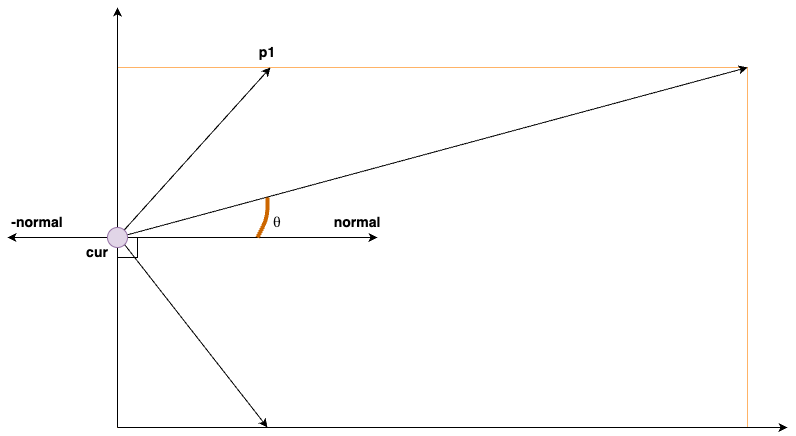
\includegraphics[width=0.8\textwidth]{../images/Normal.png}
    \caption{Внутренняя и внешняя нормали}
    \label{fig:syntdiag}
\end{figure}

Если \(\mathbf{cur}\) — граничная точка выпуклой области \(\text{polygon}\), а \(\mathbf{normal}\) — внутренняя нормаль к одной из ограничивающих эту область сторон, то для любой конкретной величины \(t\), т. е. для любой точки отрезка \(\mathbf{p0}\), \(\mathbf{p1}\):
\begin{itemize}
    \item из условия \(\mathbf{normal} \cdot (\mathbf{p}(t) - \mathbf{cur}) < 0\) следует, что вектор \(\mathbf{p}(t) - \mathbf{cur}\) направлен вовне области \(\text{polygon}\);
    \item из условия \(\mathbf{normal} \cdot (\mathbf{p}(t) - \mathbf{cur}) = 0\) следует, что \(\mathbf{p}(t) - \mathbf{cur}\) лежит в плоскости, проходящей через \(\mathbf{cur}\) и перпендикулярной нормали;
    \item из условия \(\mathbf{normal} \cdot (\mathbf{p}(t) - \mathbf{cur}) > 0\) следует, что вектор \(\mathbf{p}(t) - \mathbf{cur}\) направлен внутрь \(\text{polygon}\), как показано на рис. \ref{fig:normal2}.
\end{itemize}

\begin{figure}[H]
    \centering
    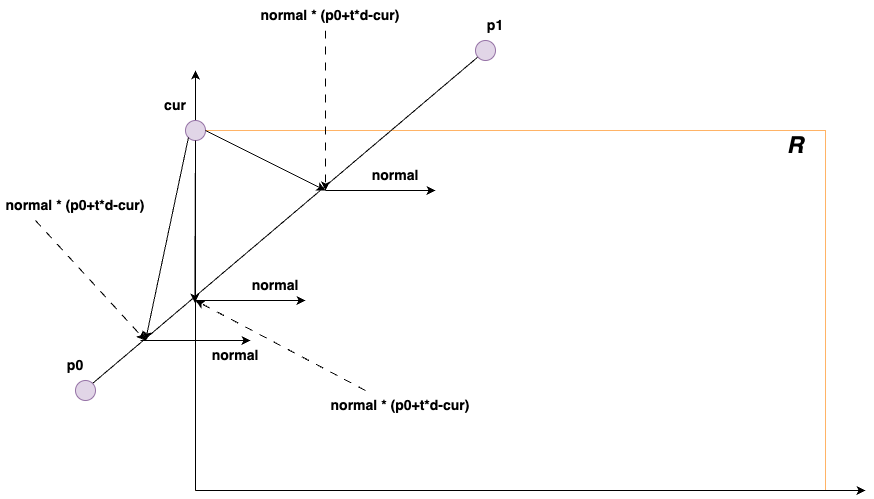
\includegraphics[width=0.8\textwidth]{../images/Normal2.png}
    \caption{Иллюстрация направлений нормалей}
    \label{fig:normal2}
\end{figure}

Из всех этих условий, взятых вместе, следует, что бесконечная прямая пересекает замкнутую выпуклую область ровно в двух точках. Далее, пусть эти две точки не принадлежат одной граничной стороне. Тогда уравнение 
\[
\mathbf{normal} \cdot (\mathbf{p}(t) - \mathbf{cur}) = 0
\]
имеет только одно решение. Если точка \(\mathbf{cur}\) лежит на той граничной стороне, для которой \(\mathbf{normal}\) является внутренней нормалью, то точка на отрезке \(\mathbf{p}\), которая удовлетворяет последнему уравнению, будет точкой пересечения этого отрезка с указанной граничной стороной.

\subsection{Расчёт параметра пересечения \(t\)}

Подставим определение для \(\mathbf{p}(t)\) в уравнение \(\mathbf{normal} \cdot (\mathbf{p}(t) - \mathbf{cur}) = 0\), получим:
\[
\mathbf{normal} \cdot \left( \mathbf{p0} + (\mathbf{p1} - \mathbf{p0})t - \mathbf{cur} \right) = 0
\iff 
\underbrace{\mathbf{normal} \cdot (\mathbf{p0} - \mathbf{cur})}_{= \text{numerator}} 
+ 
\underbrace{\mathbf{normal} \cdot (\mathbf{p1} - \mathbf{p0})}_{= \text{denominator} \ne 0} t = 0
\]
— условие пересечения отрезка с \(i\)-й границей области. Решая относительно \(t\), получим:
\[
    t = -\frac{\text{numerator}}{\text{denominator}}, \quad i = 1,2, \dots, n
\]  
Здесь \(\text{denominator} = 0\) может быть только в случае, если \(\mathbf{p1} = \mathbf{p0}\), либо если отрезок параллелен грани многоугольника.

Классификация положения точки:
\[
\text{numerator} 
\begin{cases}
< 0, & \text{точка вне многоугольника;} \\
= 0, & \text{точка на границе многоугольника;} \\
> 0, & \text{точка внутри многоугольника.}
\end{cases}
\]

Если значение \(t\) лежит за пределами интервала \(t \in [0; 1]\), то его можно проигнорировать. Хотя известно, что отрезок может пересечь выпуклый многоугольник не более чем в двух точках, уравнения могут дать большее число решений в интервале \(t \in [0; 1]\). Эти решения следует разбить на две группы: нижнюю и верхнюю, в зависимости от того, к началу или к концу отрезка будет ближе соответствующая точка. Нужно найти наибольшую из нижних и наименьшую из верхних точек. 

Если \(\text{denominator} > 0\), то найденное значение \(t\) рассматривается как возможный нижний предел. Если \(\text{denominator} < 0\), то значение \(t\) рассматривается как возможный верхний предел.
\newpage
\section{Программная реализация алгоритма Кируса-Бека}
Алгоритм был написан на языке Python 3.13.1 в интегрированной среде разработки VSCode. Для реализации графического отображения работы алгоритма использовалась библиотека matplotlib.

Инициализация параметрического представления и интервала \(t\)
\begin{lstlisting}
d = p1 - p0
t_min, t_max = 0.0, 1.0
\end{lstlisting}
\textbf{Пояснение:}  
Отрезок задаётся через точку \(\mathbf{p0}\) и вектор направления \(\mathbf{d} = \mathbf{p1} - \mathbf{p0}\). Интервал параметра \(t \in [0,1]\) соответствует всему отрезку, где \(t=0\) даёт \(\mathbf{p0}\), а \(t=1\) даёт \(\mathbf{p1}\).

Цикл по сторонам выпуклого многоугольника
\begin{lstlisting}
for i in range(n):
    cur = polygon[i]
    nxt = polygon[(i + 1) % n]
    edge_vec = nxt - cur
    normal = np.array([-edge_vec[1], edge_vec[0]], dtype=float)
\end{lstlisting}
\textbf{Пояснение:}  
Проходим по каждой стороне многоугольника. Для каждой стороны вычисляется вектор \(\mathbf{edge\_vec}\) и затем внутренняя нормаль \(\mathbf{normal} = (-\Delta y, \Delta x)\), направленная внутрь многоугольника (при условии, что вершины заданы в порядке обхода CCW).

Вычисление числителя и знаменателя для текущей стороны
\begin{lstlisting}
numerator = np.dot(normal, (p0 - cur))
denominator = np.dot(normal, d)
\end{lstlisting}
\textbf{Пояснение:}  
Здесь вычисляются:
\begin{itemize}
  \item \(\text{numerator} = \mathbf{normal} \cdot (\mathbf{p0} - \mathbf{cur})\) — определяет положение точки \(\mathbf{p0}\) относительно текущей границы.
  \item \(\text{denominator} = \mathbf{normal} \cdot \mathbf{d}\) — показывает, как направлен отрезок относительно нормали.
\end{itemize}

Обработка параллельного случая
\begin{lstlisting}
if abs(denominator) < 1e-12:
    if numerator < 0:
        return (False, None, None)
    else:
        continue
\end{lstlisting}
\textbf{Пояснение:}  
Если \(\text{denominator}\) почти равен нулю, отрезок параллелен текущей стороне. Если \(\mathbf{p0}\) находится вне (то есть \(\text{numerator} < 0\)), то отрезок не может пересечь многоугольник и алгоритм возвращает "не пересекается". Если \(\mathbf{p0}\) внутри, то эта сторона не изменяет интервал \(t\) и переходим к следующей.

Вычисление параметра \(t\) и обновление интервала \([t_{\min}, t_{\max}]\)
\begin{lstlisting}
t = - numerator / denominator
if denominator > 0:   
    if t > t_max:
        return (False, None, None)
    if t > t_min:
        t_min = t
else:               
    if t < t_min:
        return (False, None, None)
    if t < t_max:
        t_max = t

if t_min > t_max:
    return (False, None, None)
\end{lstlisting}
Здесь вычисляется значение \(t = -\frac{\text{numerator}}{\text{denominator}}\), которое соответствует точке пересечения отрезка с данной гранью. В зависимости от знака \(\text{denominator}\):
\begin{itemize}
    \item Если \(\text{denominator} > 0\) (входящая грань), обновляем \(t_{\min}\) (если \(t > t_{\min}\)).
    \item Если \(\text{denominator} < 0\) (выходящая грань), обновляем \(t_{\max}\) (если \(t < t_{\max}\)).
\end{itemize}
Если после обновления \(t_{\min} > t_{\max}\), значит пересечение отсутствует.

Вычисление итоговых точек отсечения
\begin{lstlisting}
q0 = p0 + t_min * d
q1 = p0 + t_max * d
return (True, q0, q1)
\end{lstlisting}
\textbf{Пояснение:}  
Если после обработки всех сторон интервал \([t_{\min}, t_{\max}]\) остаётся допустимым, вычисляются итоговые точки пересечения:
\[
\mathbf{q0} = \mathbf{p0} + t_{\min} \cdot \mathbf{d}, \quad \mathbf{q1} = \mathbf{p0} + t_{\max} \cdot \mathbf{d}.
\]
Эти точки и задают фрагмент отрезка, лежащий внутри многоугольника.
\newpage
\subsection{Блок-схема}
\begin{figure}[H]
    \centering
    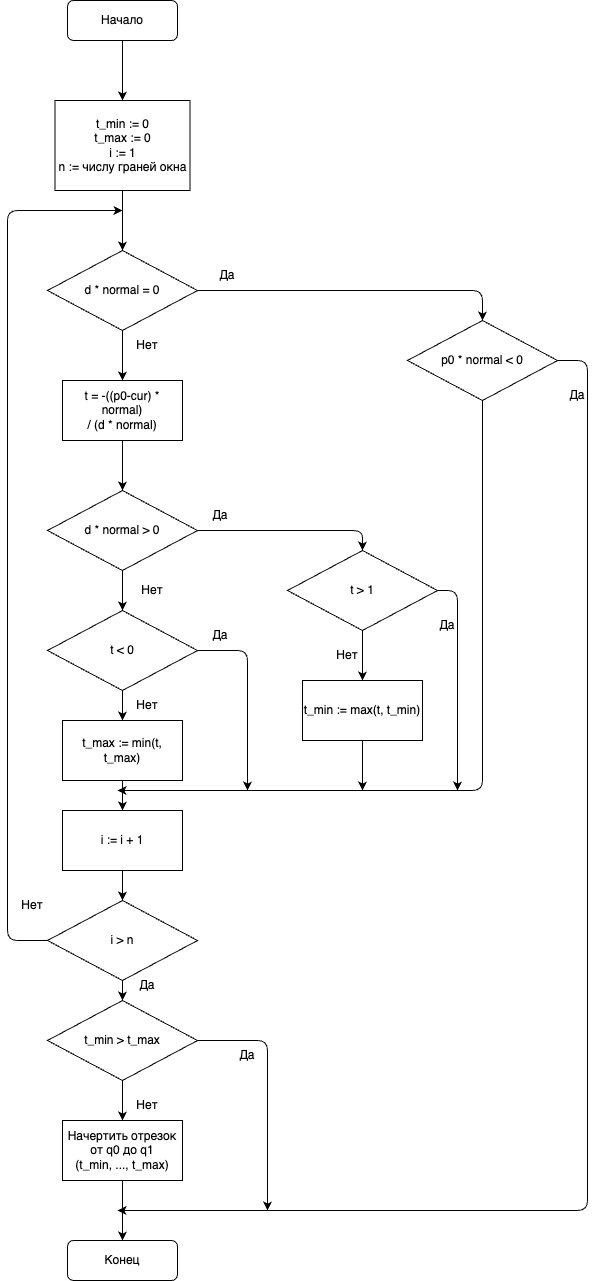
\includegraphics[width=0.6\textwidth]{../images/BlockGraphic.png}
    \caption{Блок-схема алгоритма Кируса-Бека.}
    \label{fig:blockschema}
\end{figure}

\subsection{Результаты программной реализации}
На рисунке 1 показан изначальный отрезок и выпуклый многоугольник, на рисунке 2 показано отсечение отрезка. 
\begin{figure}[H]
    \centering
    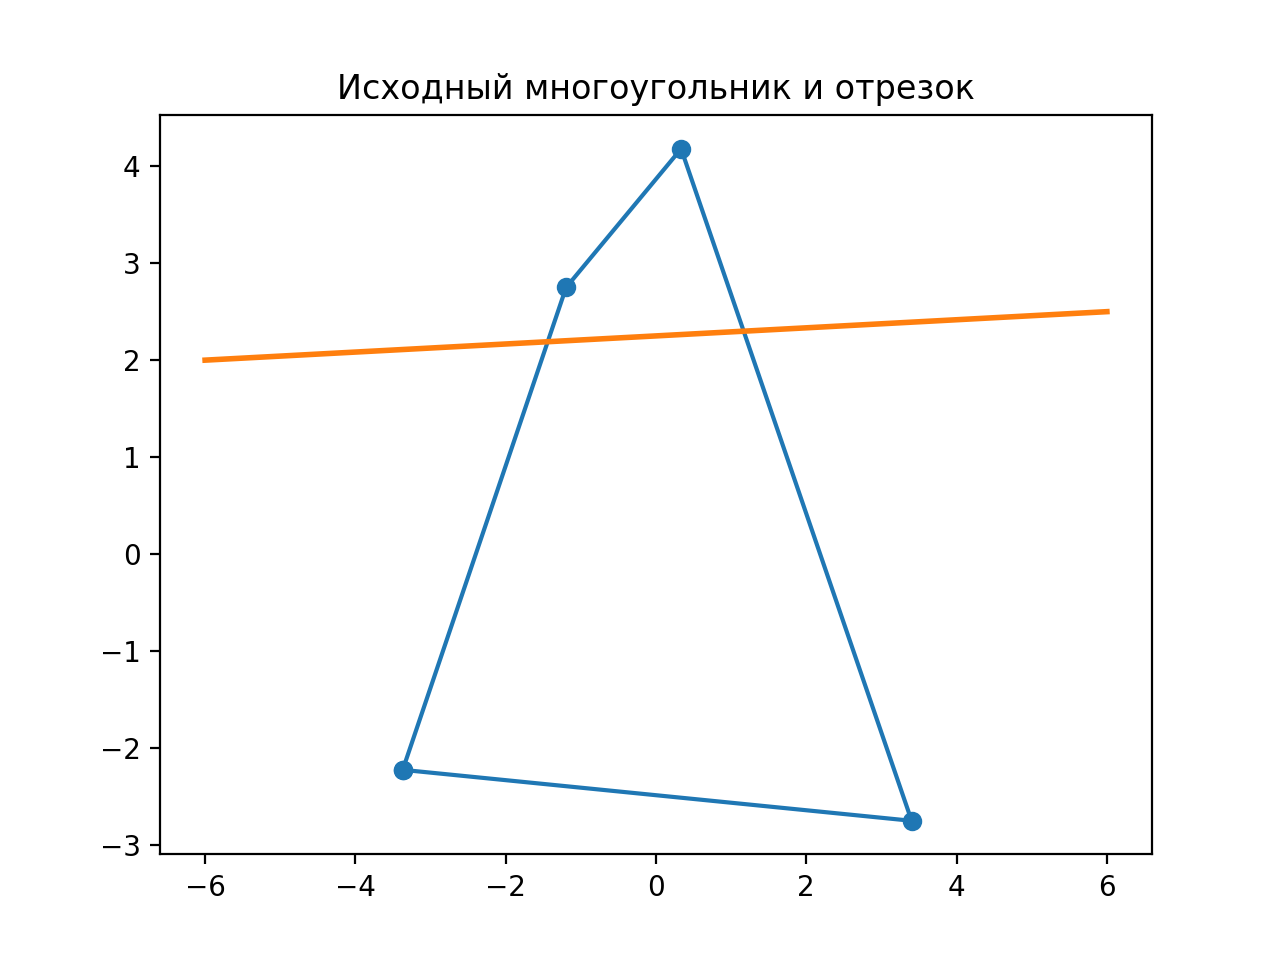
\includegraphics[width=0.5\textwidth]{../images/step1_initial.png}
    \caption{Алгоритм Кируса-Бека. Начальная стадия.}
    \label{fig:initial}
\end{figure}

\begin{figure}[H]
    \centering
    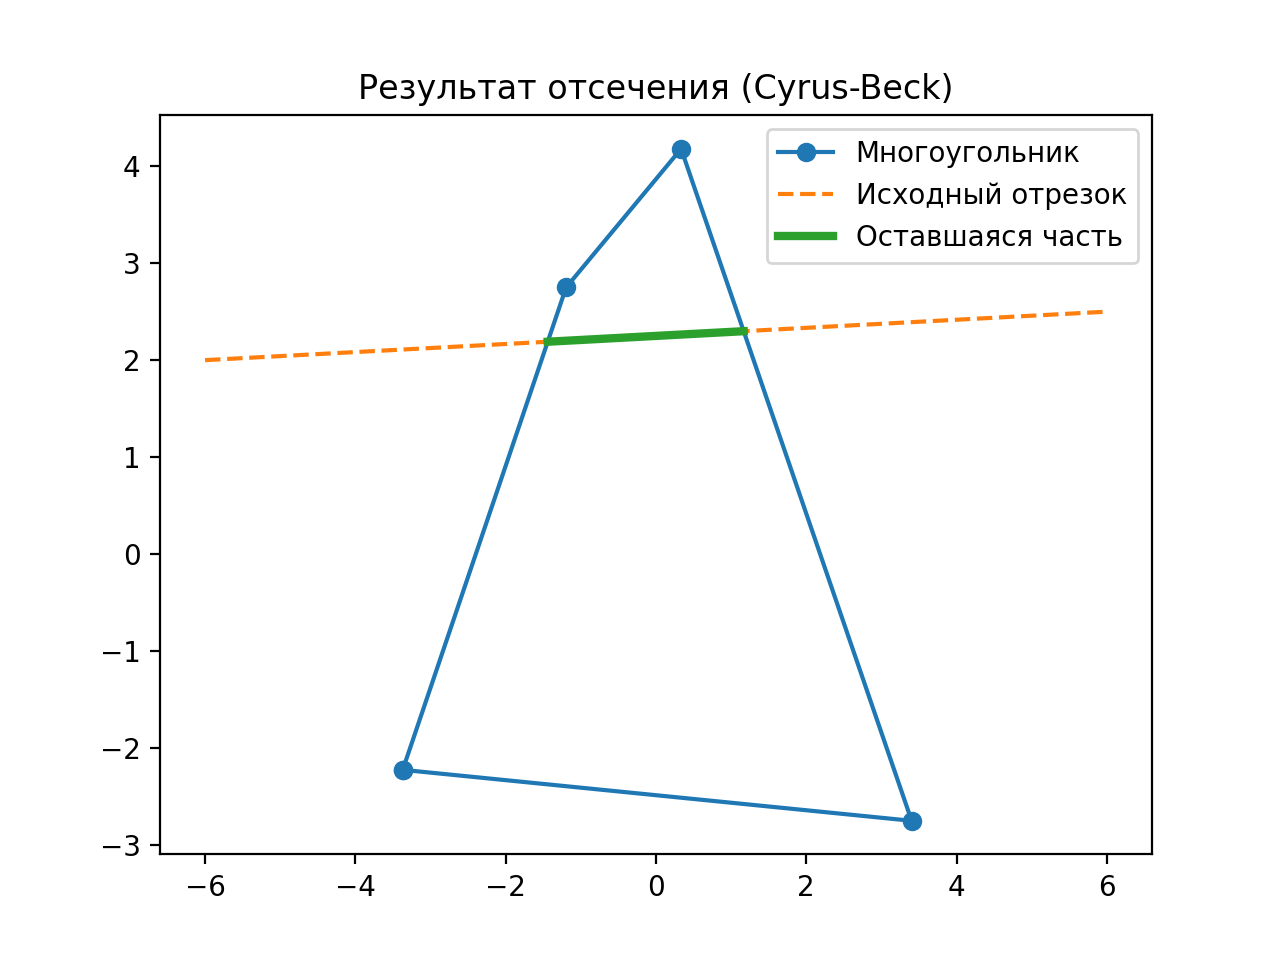
\includegraphics[width=0.5\textwidth]{../images/step3_clipped_result.png}
    \caption{Алгоритм Кируса-Бека. Полученный отрезок.}
    \label{fig:clipped}
\end{figure}
\newpage
\section{Другие алгоритмы отсечения отрезка выпуклым телом}
\subsection{Алгоритм Коэна-Сазерленда}
Алгоритм Коэна-Сазерленда изначально был разработан для отсечения линий 
прямоугольным окном (axis-aligned rectangle). Он активно использовался 
в компьютерной графике (например, при рендеринге 2D-примитивов). 
Основная идея состоит в следующем:

\begin{enumerate}
    \item Прямоугольник задаётся координатами 
    \(\text{xmin}, \text{ymin}, \text{xmax}, \text{ymax}\).
    \item Каждой точке плоскости приписывается 4-битный <<код региона>> 
    (Outcode), указывающий, где точка лежит относительно прямоугольника — 
    сверху, снизу, слева, справа. Биты (слева-справа, снизу-сверху и 
    т.\,д.). Например, используется нотация (TOP, BOTTOM, RIGHT, LEFT).
    \item Для двух концов отрезка вычисляются эти кодовые слова.
    \item \textbf{Логика отсечения:}
    \begin{itemize}
        \item Если \(\bigl(\text{код1} \mathbin{\&} \text{код2}\bigr) \neq 0\), 
        то это означает, что оба конца лежат в одной и той же 
        <<внешней>> области относительно одной из сторон 
        \(\Rightarrow\) отрезок вне, его можно сразу отбросить.
        \item Если \(\bigl(\text{код1} \mathbin{\|} \text{код2}\bigr) = 0\), 
        то это значит, что оба конца внутри прямоугольника 
        \(\Rightarrow\) отрезок целиком внутри.
        \item Иначе производится <<усечение>> одного конца, пересчитывается код, 
        повторяются проверки:
        \begin{itemize}
            \item Берётся один из концов, который находится 
            снаружи (по коду).
            \item Находится пересечение с соответствующей границей 
            прямоугольника.
            \item Заменяется этот конец на точку пересечения, 
            снова вычисляется код.
            \item Процесс повторяется, пока не станет ясно, 
            что отрезок целиком отброшен или полностью лежит внутри.
        \end{itemize}
    \end{itemize}
\end{enumerate}

Алгоритм легко реализуется, эффективно работает именно для прямоугольной 
области. Для произвольного выпуклого многоугольника он не применяется 
напрямую (без существенных модификаций).

Пример:
\begin{figure}[H]
    \centering
    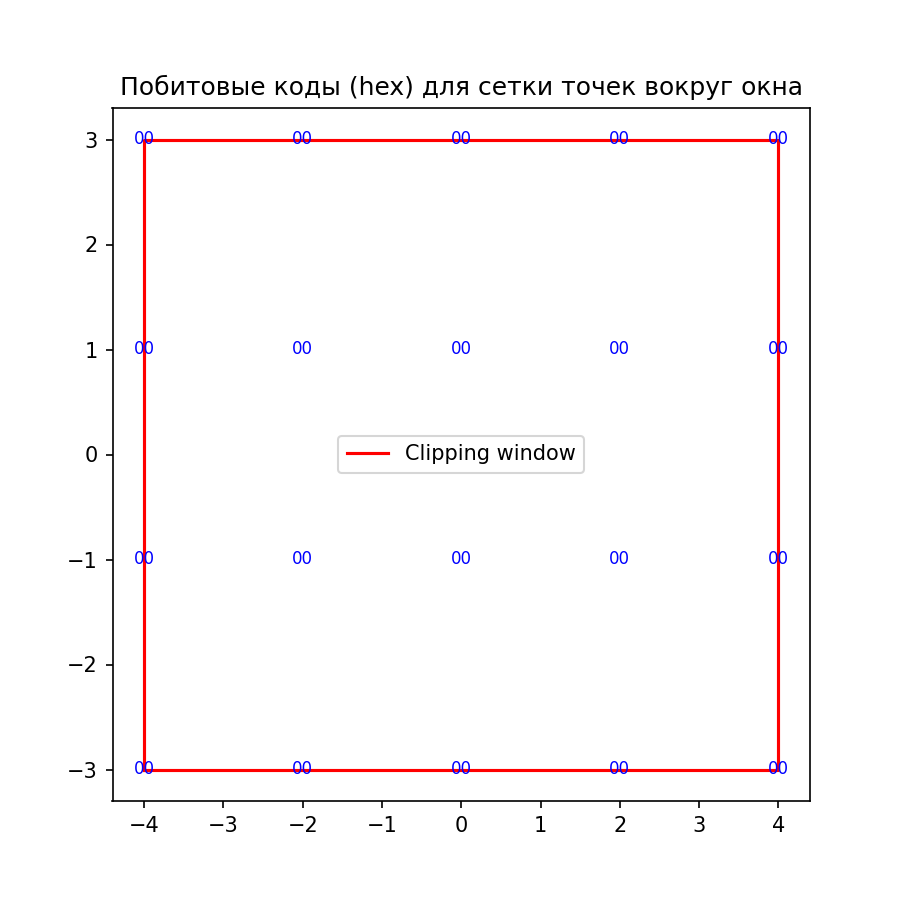
\includegraphics[width=0.5\textwidth]{../images/cohen_outcode_map.png}
    \caption{Алгоритм Коэна-Сазерленда. «Карта» побитовых кодов (Outcode) в окрестности окна отсечения.}
    \label{fig:cohen_outcode}
\end{figure}

\begin{figure}[H]
    \centering
    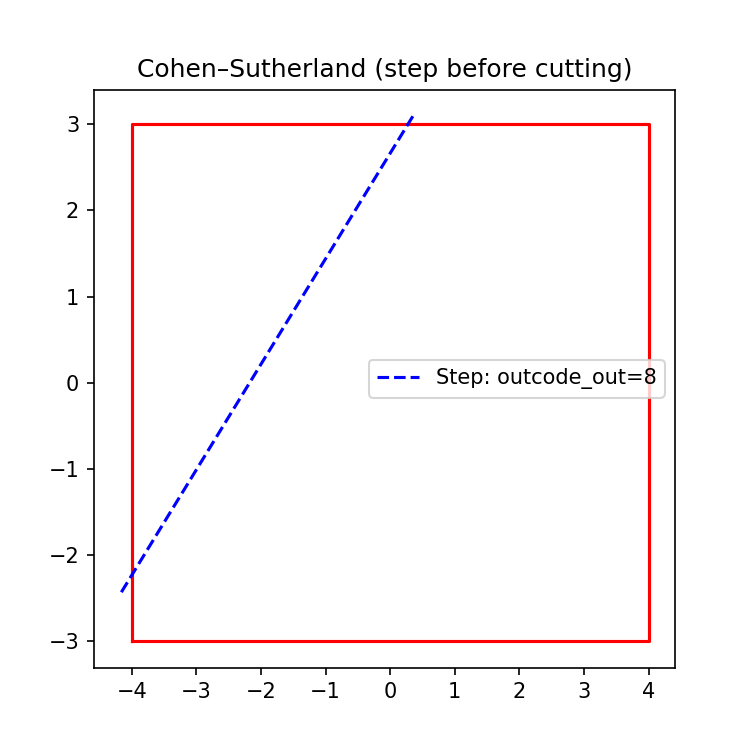
\includegraphics[width=0.5\textwidth]{../images/cohen_step_1_before.png}
    \caption{Алгоритм Коэна-Сазерленда. Промежуточное состояние до очередного «обрезания».}
    \label{fig:cohen_step1}
\end{figure}

\begin{figure}[H]
    \centering
    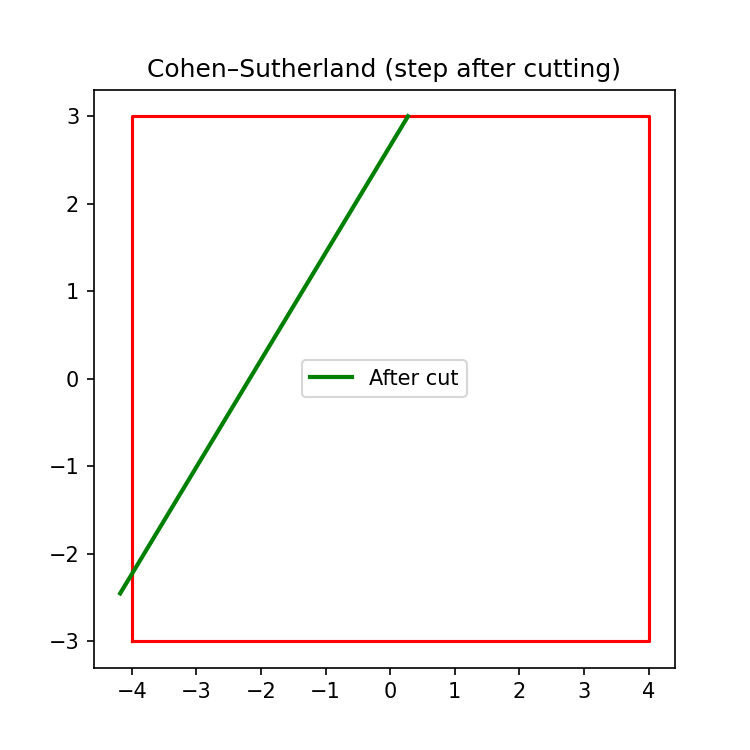
\includegraphics[width=0.5\textwidth]{../images/cohen_step_2_after.png}
    \caption{Алгоритм Коэна-Сазерленда. То же самое состояние алгоритма, но после «обрезки» одного конца.}
    \label{fig:cohen_step2}
\end{figure}

\begin{figure}[H]
    \centering
    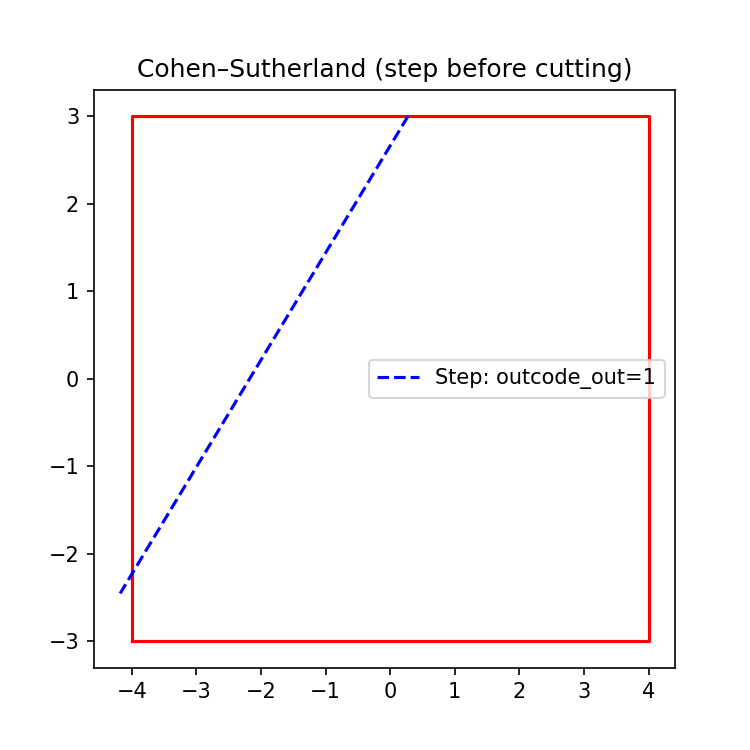
\includegraphics[width=0.5\textwidth]{../images/cohen_step_3_before.png}
    \caption{Алгоритм Коэна-Сазерленда. Промежуточное состояние до очередного «обрезания».}
    \label{fig:cohen_step3}
\end{figure}
Отсечение верхнего отрезка. 
\begin{figure}[H]
    \centering
    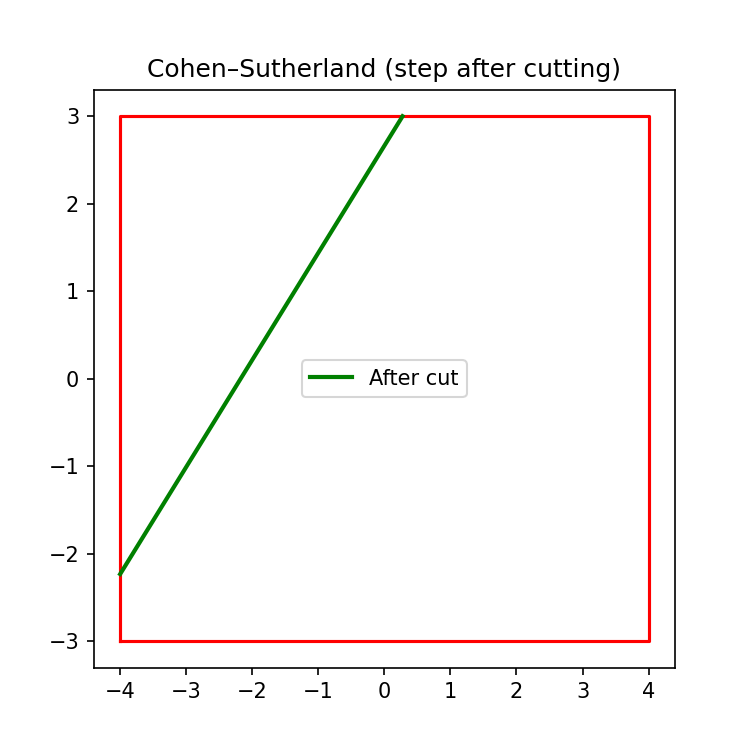
\includegraphics[width=0.5\textwidth]{../images/cohen_step_4_after.png}
    \caption{Алгоритм Коэна-Сазерленда. Промежуточное состояние после «обрезания».}
    \label{fig:cohen_step4}
\end{figure}
Конечный результат отсечения двух отрезков вне окна.
\begin{figure}[H]
    \centering
    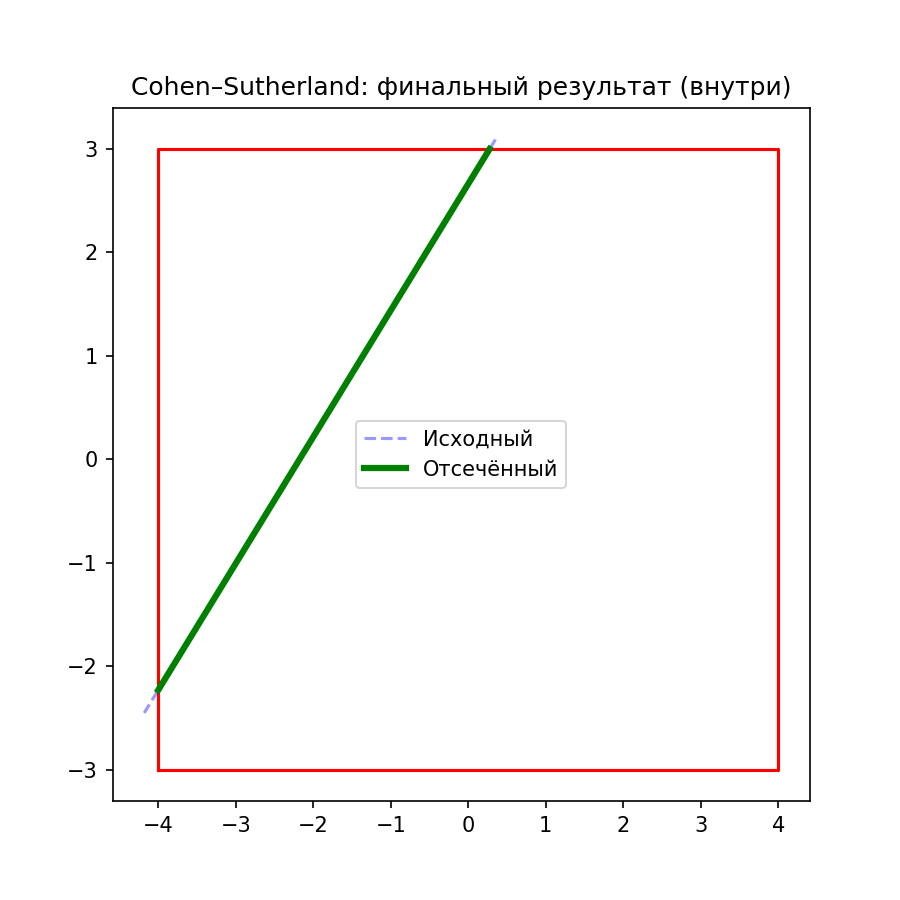
\includegraphics[width=0.5\textwidth]{../images/cohen_final_result.png}
    \caption{Алгоритм Коэна-Сазерленда. Результат.}
    \label{fig:cohen_final}
\end{figure}
\subsection{Метод пересечения с полуплоскостями}
Любое выпуклое тело в 2D (выпуклый многоугольник) можно рассматривать как 
пересечение набора полуплоскостей (каждая сторона многоугольника задаёт 
одну полуплоскость). Соответственно, чтобы отсечь отрезок, мы можем:

\begin{enumerate}
    \item Иметь список \(\{H_1,\,H_2,\,\dots,\,H_n\}\) полуплоскостей, 
    каждая определяется линейным неравенством 
    \(a_i\,x \;+\; b_i\,y \;+\; c_i \;\ge\; 0\).
    \item Начинать с <<полного>> отрезка \([\mathbf{p0},\, \mathbf{p1}]\).
    \item Для каждой полуплоскости \(H_i\) \textbf{<<обрезать>>} текущую 
    часть отрезка так, чтобы она оставалась только внутри \(H_i\). 
    Это эквивалентно вычислению пересечения отрезка с \(H_i\).
    \item Если на каком-то шаге кусок отрезка становится пустым, алгоритм 
    завершает работу (всё снаружи).
    \item В конце, если осталось что-то от отрезка, то это и есть 
    итоговое пересечение с выпуклым многоугольником.
\end{enumerate}

По сути, Кирус-Бек — это более структурированная версия 
<<пересечения с полуплоскостями>> с использованием параметра \(t\). 
Но можно реализовать этот метод и <<поэтапно>>, последовательно 
<<отрезая>> часть отрезка полуплоскостью.

Пример: 
Исходный отрезок до отсечения:
\begin{figure}[H]
    \centering
    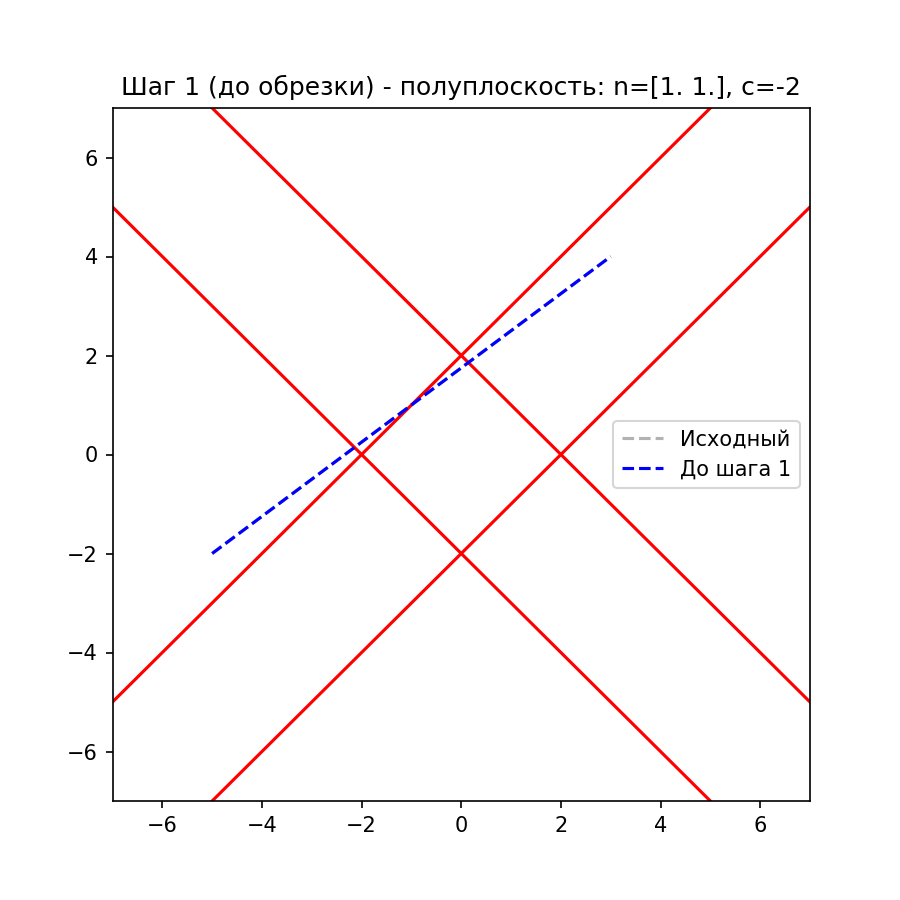
\includegraphics[width=0.5\textwidth]{../images/halfplane_step_1_before.png}
    \caption{Метод пересечения с полуплоскостями. До обрезки.}
    \label{fig:halfplane_step1}
\end{figure}
Отрезок до обрезки следующим шагом:
\begin{figure}[H]
    \centering
    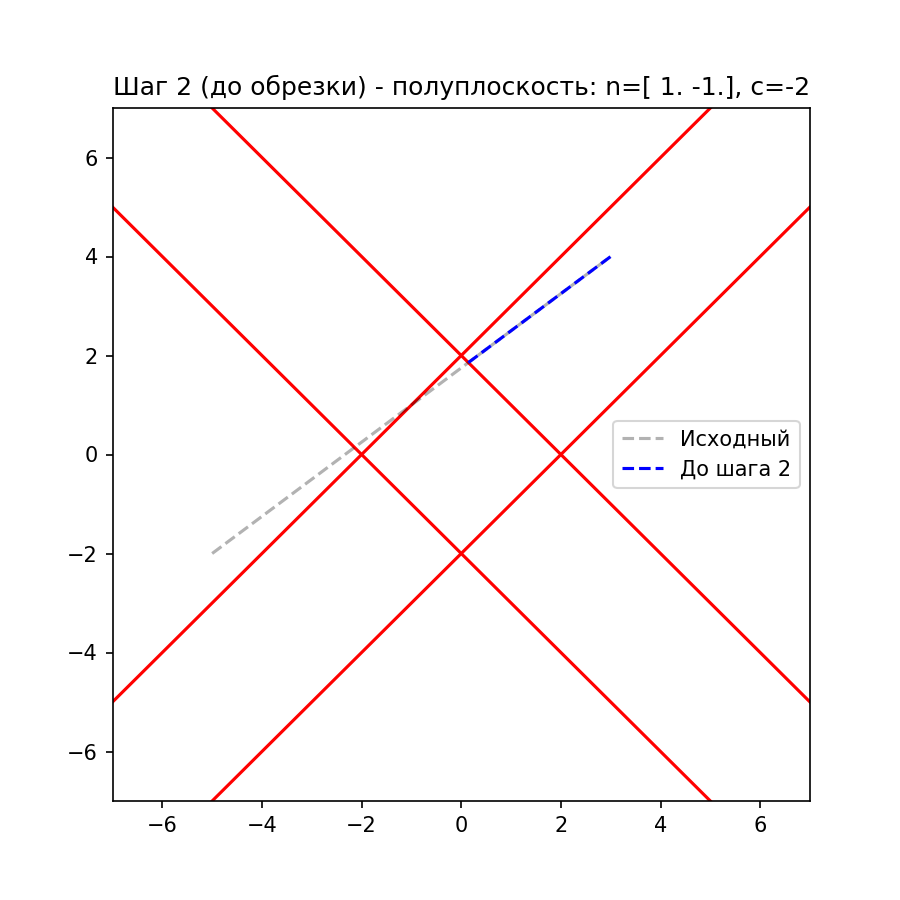
\includegraphics[width=0.5\textwidth]{../images/halfplane_step_3_before.png}
    \caption{Метод пересечения с полуплоскостями. До обрезки.}
    \label{fig:halfplane_step3}
\end{figure}
Результат обрезки отрезка:
\begin{figure}[H]
    \centering
    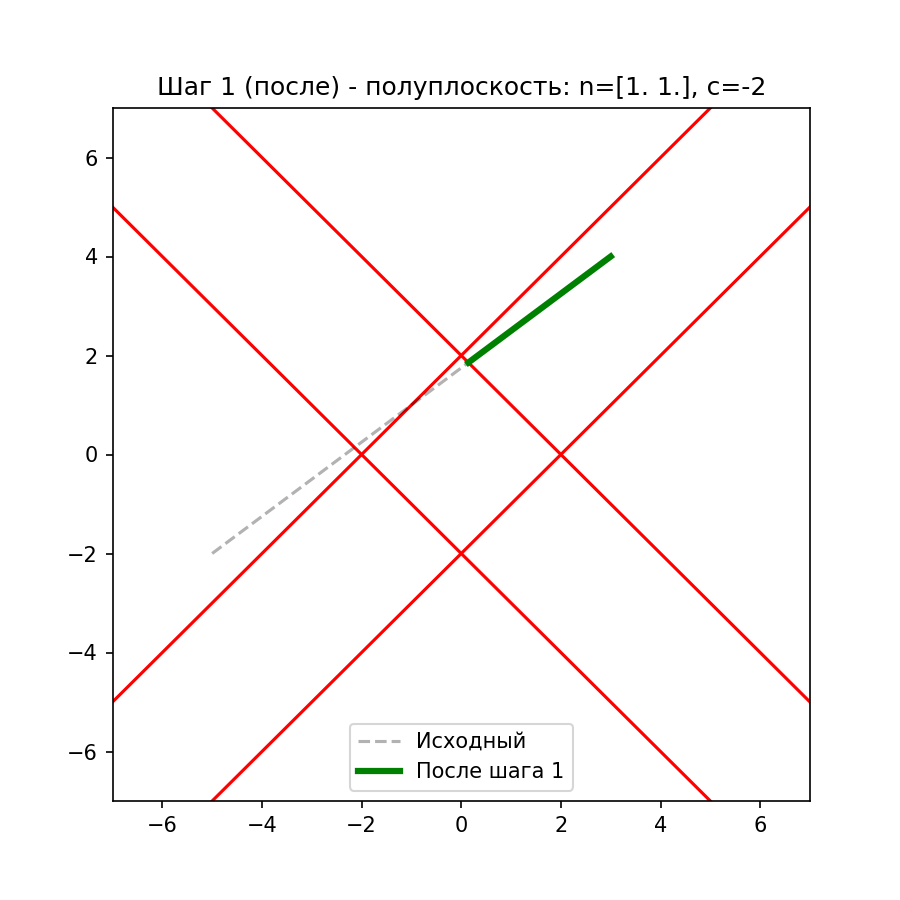
\includegraphics[width=0.5\textwidth]{../images/halfplane_step_2_after.png}
    \caption{Метод пересечения с полуплоскостями. После обрезки.}
    \label{fig:halfplane_step2}
\end{figure}
\newpage
\section{Сравнение алгоритмов}
Коэн–Сазерленд отлично подходит для отсечения отрезков прямоугольным окном благодаря использованию битовых кодов, что обеспечивает очень быструю обработку (практически \(O(1)\) для фиксированного окна). Однако алгоритм не универсален и требует значительных модификаций для произвольных выпуклых областей.

Кируса–Бека является универсальным алгоритмом, применимым для любого выпуклого многоугольника (и даже для 3D), но его сложность составляет \(O(n)\), что может стать узким местом при большом числе сторон.

Метод пересечения с полуплоскостями по сути эквивалентен Кируса–Бека в плане функциональности и сложности (\(O(n)\)). Он концептуально проще, так как сводится к последовательному «подрезанию» отрезка по каждой полуплоскости, но на практике его реализация будет схожа по сложности и особенностям с алгоритмом Кируса–Бека.

Таким образом, выбор алгоритма зависит от конкретной задачи: для простых прямоугольных окон эффективен Коэн–Сазерленд, а для произвольных выпуклых областей лучше использовать Кируса–Бека или метод пересечения с полуплоскостями.

\newpage
\section{Сравнение собственной реализации с библиотечной}
В библиотечной версии языка Python алгоритмом, аналогичным Кируса-Бека, является алгоритм Shapely. Было проведено 500 тестов. 
\begin{table}[h!]
    \centering
    \caption{Сравнение производительности алгоритма Cyrus–Beck и библиотеки Shapely}
    \label{tab:performance}
    \begin{tabular}{cccccc}
    \toprule
    Сценарий & Тестов & Вершин & Радиус & Cyrus–Beck (мкс) & Shapely (мкс) \\
    \midrule
    1 & 500 & 10  & 10 & 15.48 & 41.70 \\
    2 & 500 & 30  & 10 & 28.63 & 40.30 \\
    3 & 500 & 50  & 10 & 46.48 & 88.04 \\
    4 & 500 & 100 & 15 & 30.62 & 35.06 \\
    \bottomrule
    \end{tabular}
\end{table}
Где Cyrus-Beck — реализация собственного алгоритма. 
Как было сказано во введении, наша реализация уступает библиотечной при малых \(n\) и незначительно уступает при больших \(n\). 
Ниже представлена гистограмма сравнения.
\begin{figure}[H]
    \centering
    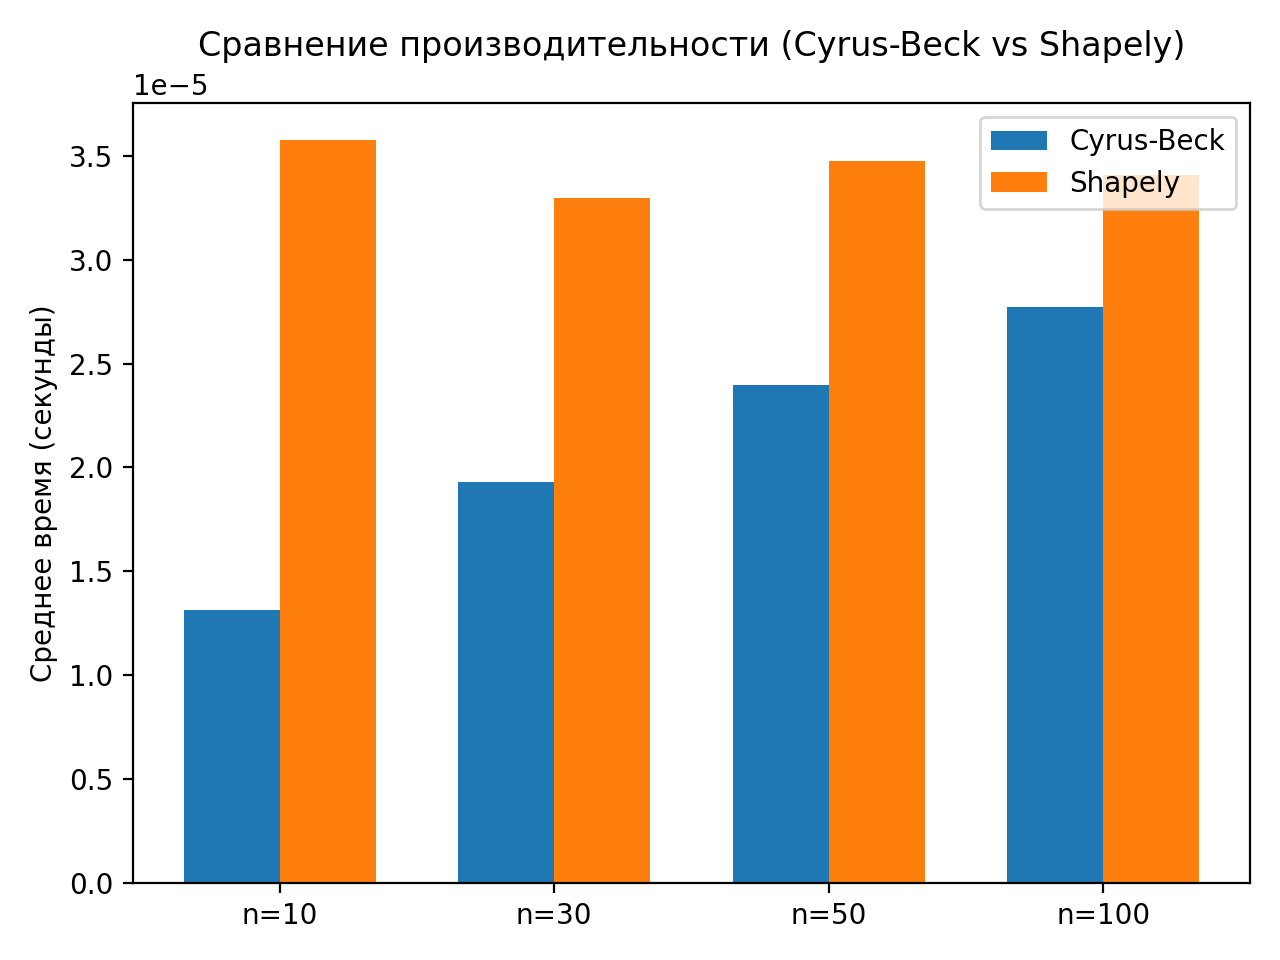
\includegraphics[width=0.5\textwidth]{../images/comparison_cyrus_vs_shapely.png}
    \caption{Сравнение собственной реализации с Shapely.}
    \label{fig:comparison}
\end{figure}
\newpage
\section*{Заключение}
\addcontentsline{toc}{section}{Заключение}
В данной лабораторной работе был изучен и реализован алгоритм отсечения отрезка выпуклым телом. Также были изучены и рассмотрены другие алгоритмы отсечения отрезка выпуклыми телами, такие как:
\begin{itemize}
    \item Алгоритм Коэна-Сазерленда
    \item Метод пересечения с полуплоскостями
\end{itemize}
Математически был описан алгоритм Кируса-Бека, в последствии реализации было проведено сравнение с библиотечным аналогом алгоритма Shapely. Для реализации теста было создано 4 сценария по 500 тестов с разным числом вершин (\(n\)). В результате сравнения библиотечный аналог оказался быстрее нашего алгоритма, поскольку Shapely имеет реализацию на более низкоуровневом языке программирования, однако сложность обоих алгоритмов одинакова: \(O(n)\). 
\newpage
\section*{Список литературы}
\addcontentsline{toc}{section}{Список литературы}
\begin{enumerate}
    \item Препарата Ф., Шеймос М., "Вычислительная геометрия: введение"
\end{enumerate}
\newpage
\section*{Приложение А}
\addcontentsline{toc}{section}{Приложение А}
\begin{lstlisting}
import random
import time
import numpy as np
import matplotlib.pyplot as plt

try:
    from shapely.geometry import Polygon, LineString
    shapely_available = True
except ImportError:
    shapely_available = False

def convex_hull(points):
    points = sorted(points, key=lambda p: (p[0], p[1]))

    def cross(o, a, b):
        return (a[0] - o[0])*(b[1] - o[1]) - (a[1] - o[1])*(b[0] - o[0])

    lower = []
    for p in points:
        while len(lower) >= 2 and cross(lower[-2], lower[-1], p) <= 0:
            lower.pop()
        lower.append(p)

    upper = []
    for p in reversed(points):
        while len(upper) >= 2 and cross(upper[-2], upper[-1], p) <= 0:
            upper.pop()
        upper.append(p)

    lower.pop()
    upper.pop()
    hull = lower + upper
    return np.array(hull)

def generate_random_convex_polygon(num_points=7, radius=5):
    points = []
    for _ in range(num_points):
        r = radius * random.random()**0.5
        theta = 2 * np.pi * random.random()
        x = r * np.cos(theta)
        y = r * np.sin(theta)
        points.append((x, y))
    hull = convex_hull(points)
    return hull

def is_segment_outside_bounding(p0, p1, polygon):
    poly_x = polygon[:, 0]
    poly_y = polygon[:, 1]
    min_x, max_x = min(poly_x), max(poly_x)
    min_y, max_y = min(poly_y), max(poly_y)

    seg_x = [p0[0], p1[0]]
    seg_y = [p0[1], p1[1]]
    seg_min_x, seg_max_x = min(seg_x), max(seg_x)
    seg_min_y, seg_max_y = min(seg_y), max(seg_y)

    if seg_max_x < min_x or seg_min_x > max_x:
        return True
    if seg_max_y < min_y or seg_min_y > max_y:
        return True
    return False

def cyrus_beck_clip(p0, p1, polygon):
    d = p1 - p0
    t_min, t_max = 0.0, 1.0
    n = len(polygon)

    for i in range(n):
        cur = polygon[i]
        nxt = polygon[(i + 1) % n]
        edge_vec = nxt - cur
        normal = np.array([-edge_vec[1], edge_vec[0]], dtype=float)  
        numerator   = np.dot(normal, (p0 - cur))
        denominator = np.dot(normal, d)

        if abs(denominator) < 1e-12:
            if numerator < 0:
                return (False, None, None)  
            else:
                continue  

        t = - numerator / denominator
        if denominator > 0:
            if t > t_max:
                return (False, None, None)
            if t > t_min:
                t_min = t
        else:
            if t < t_min:
                return (False, None, None)
            if t < t_max:
                t_max = t

        if t_min > t_max:
            return (False, None, None)

    if t_max < 0 or t_min > 1:
        return (False, None, None)

    q0 = p0 + t_min * d
    q1 = p0 + t_max * d
    return (True, q0, q1)

def clip_segment_with_cyrus_beck(p0, p1, polygon):
    if is_segment_outside_bounding(p0, p1, polygon):
        return (False, None, None)
    return cyrus_beck_clip(p0, p1, polygon)

def shapely_clip(p0, p1, polygon):
    poly  = Polygon(polygon)
    line  = LineString([p0, p1])
    inter = poly.intersection(line)
    if inter.is_empty:
        return (False, None, None)
    if inter.geom_type == 'LineString':
        coords = list(inter.coords)
        q0 = np.array(coords[0])
        q1 = np.array(coords[-1])
        return (True, q0, q1)
    if inter.geom_type == 'Point':
        q = np.array(inter.coords[0])
        return (True, q, q)
    if inter.geom_type == 'MultiPoint':
        coords = sorted([np.array(pt.coords[0]) for pt in inter.geoms], key=lambda x: (x[0], x[1]))
        return (True, coords[0], coords[-1])
    return (True, None, None)

def compare_performance(num_tests=1000, polygon_size=30, radius=10):
    polygon = generate_random_convex_polygon(num_points=polygon_size, radius=radius)

    cyrus_times = []
    shapely_times = []
    
    for _ in range(num_tests):
        p0 = np.array([random.uniform(-2*radius, 2*radius),
                       random.uniform(-2*radius, 2*radius)])
        p1 = np.array([random.uniform(-2*radius, 2*radius),
                       random.uniform(-2*radius, 2*radius)])
        
        start = time.perf_counter()
        res1 = clip_segment_with_cyrus_beck(p0, p1, polygon)
        end = time.perf_counter()
        cyrus_times.append(end - start)

        if shapely_available:
            start = time.perf_counter()
            res2 = shapely_clip(p0, p1, polygon)
            end = time.perf_counter()
            shapely_times.append(end - start)
        else:
            shapely_times.append(float('nan'))

    mean_cyrus   = np.mean(cyrus_times)
    mean_shapely = np.mean([t for t in shapely_times if not np.isnan(t)])
    return mean_cyrus, mean_shapely

def demo_comparison():
    scenarios = [
        (500,  10,  10),
        (500,  30,  10),
        (500,  50,  10),
        (500, 100, 15),
    ]
    
    cyrus_results = []
    shapely_results = []
    labels = []

if __name__ == "__main__":
    demo_comparison()

\end{lstlisting}
\end{document}